\documentclass[a4paper]{article}
\usepackage[utf8]{inputenc}
\usepackage[english]{babel}
\usepackage[babel=true]{csquotes}
\usepackage{graphicx}

\pagestyle{headings}

\title{Computer Network Architectures and Multimedia: Assignement 1}
\author{Julien Nix and Raphaël Javaux}
\date{}

\begin{document}
\maketitle

 \section{Question 1}

   \subsection{TCP behavior}

    \paragraph{}TCP starts sending by packet at a time, waiting for a single ACK.
By increasing the transmission window size, TCP gets its maximum throughput
after around 0.5 second.

   \subsection{n0 to n1 throughput}

    \paragraph{}TCP achives a constant 2.7 Mbps/sec throughput during the last
3 seconds, which is quite close to the half of the bandwidth of the links
(6 Mbps).
This confirms our previous observation that TCP Tahoe reaches its maximum
throughput after half a second.

    \paragraph{}The script can be run with this command :
    \begin{verbatim}
        runhaskell Q1_2.hs < Q1_1.tr
    \end{verbatim}

   \subsection{n0 to n2 falls down}

   \paragraph{}Every packet which was on the n0 to n2 link has been lost.
New packets have been redirected to n2 over the n0 to n1 link (which is already
used by the TCP flow), resulting in the n0's queue overflow.

    \paragraph{}As TCP detected the loss of packets, it promptly restarted its
congestion detection algorithm to accommodates itself to the new available
bandwidth of the n0 to n1 link.

   \subsection{Network recovery}
   \label{Network recovery}

   \paragraph{}The last packet drop happened at 3.23 sec, but TCP only recovers
an ideal throughput around 3.6 sec, after a few iterations of its congestion
detection algorithm.

   \subsection{Packets dropped}

   \paragraph{}TCP flow packets dropped: 1
   \paragraph{}UDP flow packets dropped: 14

    \paragraph{}The script can be run with this command :
    \begin{verbatim}
        runhaskell Q1_5.hs < Q1_3.tr
    \end{verbatim}

   \subsection{Throughput graph}

    \begin{center}
        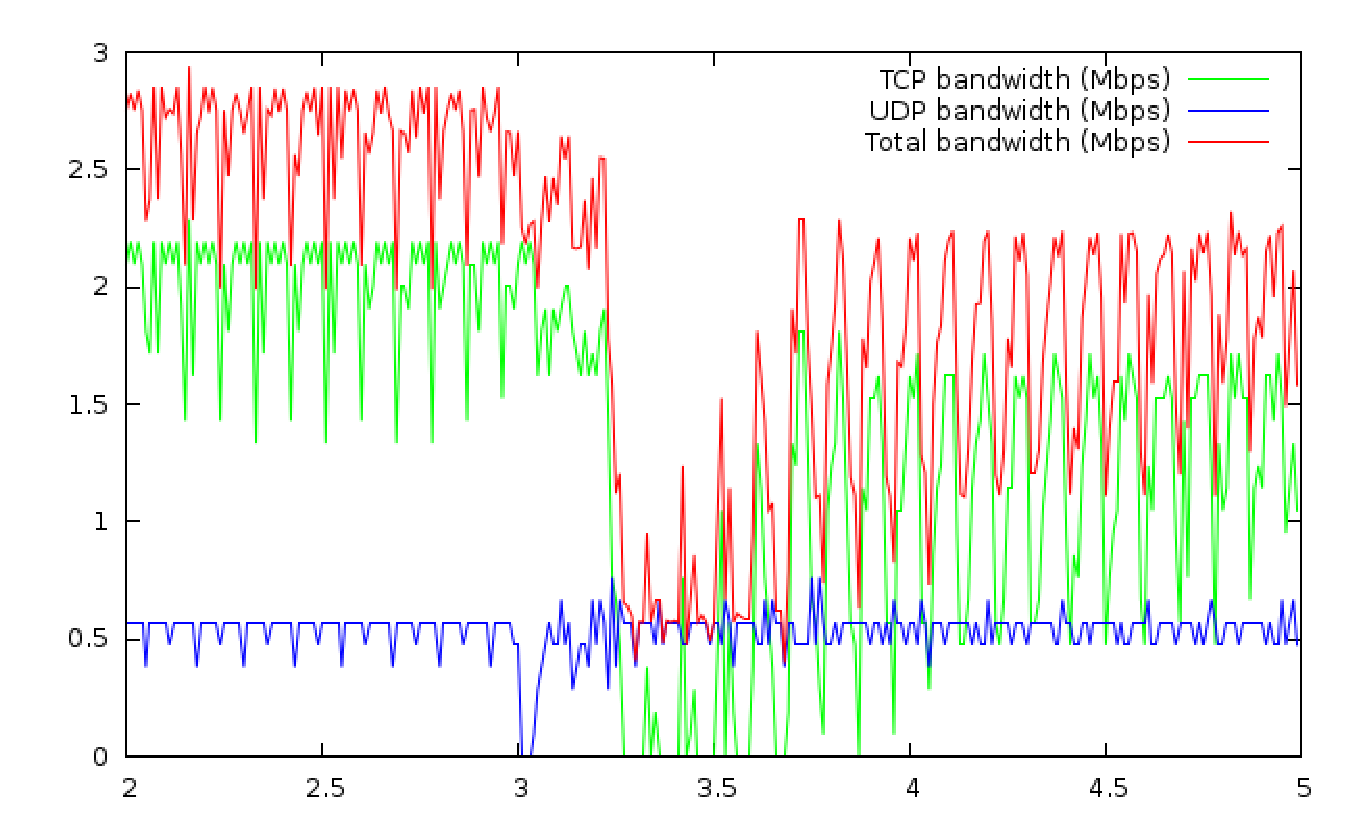
\includegraphics[width=\textwidth]{question1/Q1_6.eps}
    \end{center}

    \paragraph{}All along the simulation, we can see TCP Tahoe running its
congestion-avoidance algorithm. \newline
Soon after 3.0 sec, when the n0 to n2 link falls down, TCP reinitialised its
sending window and its congestion-detection algorithm. As said in
\ref{Network recovery}, TCP recovered an ideal throughput shortly after 3.5 sec
and correctly took into account the new UDP traffic on the n0 to n1 link.

    \paragraph{}The script can be run with this command :
    \begin{verbatim}
        runhaskell Q1_6.hs < Q1_3.tr | gnuplot --persist
    \end{verbatim}

\end{document}